%!TEX root = proj_report_outline.tex
\chapter{Evaluation}
Following the completed implementation and infrastructure setup an evaluation of the project was carried out on prototype. The evaluation was designed primarily to verify whether or not the prototype developed was successful in fulfilling the requirements identified as in scope in Section \ref{S:evaluationScope}.

\section{Experiment \rom{1} - Collaboration Functionality Fulfilment}

\subsection{Motivation}
PitchHub's primary goal is to facilitate collaboration within in the innovation community. To do this PitchHub seeks to engage all roles in the innovation community by focusing de-constructing ideas to appeal their expertise - in terms of  value proposition, business opportunity, challenges, and solution. Experiment \rom{1} seeks to verify that the prototype supports the behaviour necessary to facilitate this collaboration. As discussed in Section \ref{C:requirements} this behaviour is distilled in the requirements D1, D2.1 and D2.2.

\subsection{Results}
The user stories which affirm the fulfilment of requirements D1, D2.1 and D2.2 in \textit{TB1} confirm support of the following behaviour:

\paragraph{Requirement D1's user stories specify the ability to:} post Pitch Cards, make suggestions on Pitch Points, accept/reject suggestions, comment on Pitch Points, comment on suggestions and mark Pitch Cards as completed/active.

\paragraph{Requirement D2.1's user stories specify the ability to:} scope entities such as Pitch Cards, suggestions, and one's identity such that unintended viewers are avoided. To ensure the completeness of these user stories, each scope/viewer level combination is tested. These combinations are displayed in Fig \ref{fig:architecturescope_matrix_evaluation}.

\begin{figure}[ht]
    \centering
    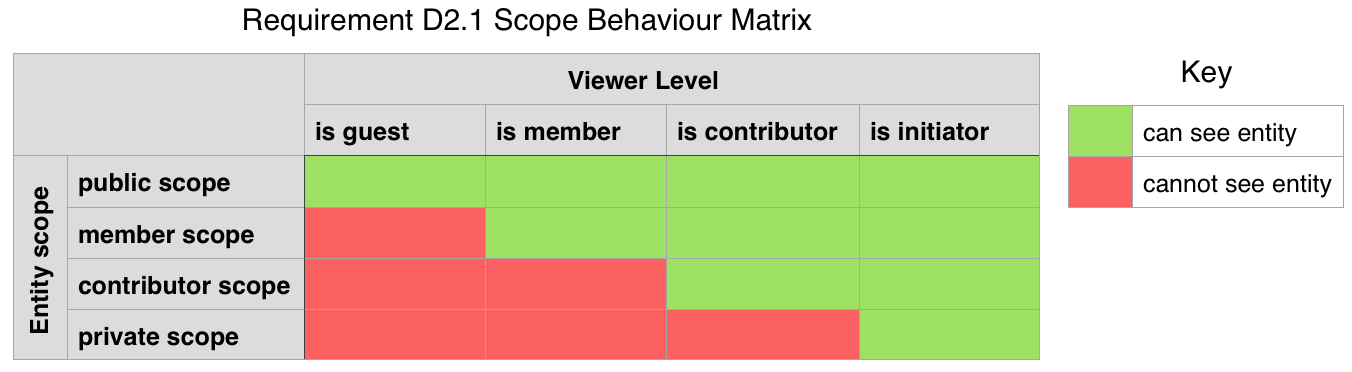
\includegraphics[width=1\textwidth]{scope_matrix}
    \caption{The scope matrix which illustrates the relationship between viewer level and entity scope in regards to viewing the entity.}
    \label{fig:architecturescope_matrix_evaluation}
\end{figure}

\paragraph{Requirement D1's user stories specify that:} users who have viewed a Pitch Card are able to be seen as a ``viewer'' by the PitchCard's initiator.

\subsection{Discussion}
The design of this experiment was guided by two main questions: first, ``what behaviours are needed to facilitate collaboration in the innovation community?'' And second, ``how can these behaviours be verified as functional from a user\'s point of view?''. In regards to the first question, determining what behaviours were required was to an extent already completed by Callaghan Innovation through their conceptualisation of PitchHub. To formalise these behaviours Callaghan Innovation and I collaborated on the specification of the user stories.
In regards to the second question, realistically simulating user interaction was identified as key. Manually testing the various behaviours and scope combinations would be time-consuming and tedious. \textit{TB1} automates this simulation with the added benefit of assertions, making it possible verify that expected behaviour is indeed satisfied.
Concluding on the fulfilment of requirements D1, D2.1 and D2.2 largely relies on whether the behaviours specified in relation to the first question accurately reflects the behaviour required by the innovation community. Generalising what a large population needs is a difficult task but it is my belief that because the user stories tested were created in collaboration with Callaghan Innovation, who is a large participant in the innovation community, they are therefore meet the level of credibility required for the purposes of this experiment. As such, it is concluded that requirements D1, D2.1 and D2.2 have been fulfilled.

\section{Experiment \rom{2} - Deployed Prototype Analysis}
At the time of writing, the prototype, \textit{TB3}, has been successfully been released to Callaghan Innovation and is ready for use. Unfortunately use of the prototype by Callaghan Innovation has not yet fully commenced. Without substantial activity to analyse this experiment was unable to be completed. It is expected that the access code will be distributed by the Callaghan Innovation stakeholders to the wider organisation in the coming weeks.

\section{Response Time Thresholds}
The following experiments explore the performance of the PitchHub prototype under various configurations using \textit{TB2}. The measure upon which performance quality is based on Nielsen and Miller's response time thresholds \cite{Responsetime:online} for web application performance. 
The response time thresholds are as follows:
\paragraph{0.1 second} is about the limit for having the user feel that the system is reacting instantaneously, meaning that no special feedback is necessary except to display the result.
\paragraph{1.0 second} is about the limit for the user's flow of thought to stay uninterrupted, even though the user will notice the delay. Normally, no special feedback is necessary during delays of more than 0.1 but less than 1.0 second, but the user does lose the feeling of operating directly on the data.
\paragraph{10 seconds} is about the limit for keeping the user's attention focused on the dialogue. For longer delays, users will want to perform other tasks while waiting for the computer to finish, so they should be given feedback indicating when the computer expects to be done. Feedback during the delay is especially important if the response time is likely to be highly variable, since users will then not know what to expect.

\section{Experiment \rom{3} - Size of Community Comparison}

\subsection{Motivation}

\subsection{Results}

\subsection{Discussion}

\section{Experiment \rom{4} - Overhead of Threshold Scheme Security}

\subsection{Motivation}

\subsection{Results}

\subsection{Discussion}

\section{Experiment \rom{5} - Overhead of Secret Keeper Diversity}

\subsection{Motivation}

\subsection{Results}

\subsection{Discussion}


\section{General Discussion}

A limitation of the experiment described in Section \ref{SS:performance} is that it is only semi-globally distributed. Two servers hosted on AWS (located in Oregon, USA) and two servers hosted by Callaghan Innovation in Wellington provide an uncommon network topology. The Secret Sharing Service with the ``3, 4'' threshold scheme means that on each database query at least one request will be sent to one of the AWS instances. This impacts the performance results due to the latency incurred. For performance results it would have been better to have all servers hosted within New Zealand. However, security and disaster recovery considerations motivated the move to embrace a more geographically distributed network.

The disadvantage of unconditionally secure secret sharing schemes is that the storage and transmission of the shares requires an amount of storage and bandwidth resources equivalent to the size of the secret times the number of shares. If the size of the secret were significant, say 1 GB, and the number of shares were 10, then 10 GB of data must be stored by the shareholders
